\providecommand{\main}{..}		% Override relative path to the main file (already set in main file)
\documentclass[../InterneDSLs.tex]{subfiles}
\begin{document}

\chapter{Bau des Prototypen}

\section{Aufbau}
Die Verarbeitung der Grammatik erfolgt nach dem folgenden Schema:
\begin{itemize}
	\item Parsen der Grammatik
	\item Aufbau des Syntax-Baumes (aus Java-Typen)
	\item Abbildung in einen Graphen, der die Aufrufreihenfolge abbildet
	\item Generierung der Interfaces
\end{itemize}

\section{Parser}
Als Parser-Generator wurde ANTLR4 verwendet, der Parser zu einer EBNF-Grammatik in Java generieren kann. Dafür verwendet ANTLR aber eine unübliche Syntax, die sich an einer alten EBNF-Variante orientiert.

Der von ANTLR generierte Parser wird von einem Listener erweitert, der aus den EBNF-Konstrukten (die praktisch Strings entprechen) einen Baum aus eigenen Klassen generiert. Dadurch wird eine Typ-Sicherheit hergestellt, die durch die EBNF selbst nicht gegeben ist.

\section{Abbildung von EBNF auf Interfaces}
Zuerst wird die in EBNF geschriebene Grammatik in einen Baum aus Java-Objekten transformiert. Dadurch wird eine Typ-Sicherheit hergestellt und Methoden implementiert werden, die das Traversieren des Baumes vereinfachen. Abbildung~\ref{FIG:TypesBNF} zeigt die Typen und ihre Beziehungen untereinander. Diese Typen finden sich auch in den Regeln der EBNF-Grammatik (Abbildung~\ref{LST:EBNFGrammar}) wieder.

Danach wird aus dem Baum ein Graph generiert, der eine Abfolge aus Knoten und Kanten darstellt. Die Knoten repräsentieren die Scopes (die durchnummerierte Namen erhalten), die Kanten repräsentierten die Methoden. In den folgenden Abschnitten wird die Abbildung der EBNF-Konstrukte auf die des Graphen und Interfaces erklärt.

Zum Erstellen des Graphen wird die Bibliothek JGraphT\cite{JGraphT} verwendet. Sie bietet verschiedene Arten von Graphen aus der Graphentheorie mit dazugehörigen Algorithmen und Konsistenzregeln an. Die Bibliothek wird aktiv weiterentwickelt und benötigt Java ab Version 1.8.

Für diesen Anwendungsfall wird ein gerichteter Pseudo-Graph, der mehrere Kanten zwischen zwei Knoten erlaubt; mehrere Kanten werden bei optionalen Elementen und Schleifen benötigt.


\begin{figure}[ht]
\centering
\includegraphics[width=\linewidth]{\main/10_Pictures/BNF-Types}
\caption{Typen des BNF-Baumes}
\label{FIG:TypesBNF}
\end{figure}

\subsection{Kante mit einem Knoten}
Der einfachste Fall ist der von einer Sequenz, die nur ein Element beinhaltet. Hier kann das Element auf eine Kante zwischen zwei Knoten abgebildet werden. Die Namen der Scopes werden zu den Interfaces, bzw. zum Rückgabewert der Methode, deren Namen dem der der Kante entspricht. Grafik~\ref{FIG:OneElementNode} zeigt, wie eine Abbildung aussehen kann.
\begin{figure}[ht]
\centering
  \begin{subfigure}[c]{0.49\textwidth}
  	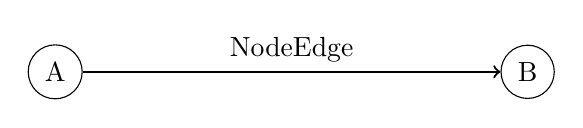
\begin{tikzpicture}
		\tikzset{vertex/.style = {shape=circle,draw,minimum size=.2em}}
		\tikzset{edge/.style = {->,> = latex'}}
		\node[vertex] (a) at  (0,0) {A};
		\node[vertex] (b) at  (6,0) {B};
		\path[->,draw,thick] (a) edge node[above] {NodeEdge} (b);
	\end{tikzpicture}
    \caption{Diagramm eines Sequenz-Knotens}
    \label{FIG:DiagramOneElementNode}
  \end{subfigure}
  \begin{subfigure}[c]{0.49\textwidth}
    \lstinputlisting[language=Java,caption={Java-Interface aus einem Sequenz-Knoten},label={LST:JInterfaceOneElementNode}]{Scope_one-element.java}
  \end{subfigure}
  \caption{Diagramm und Interface eines Sequenz-Knotens}
  \label{FIG:OneElementNode}
\end{figure}

Im Falle eines optionalen Elementes, muss auch der Methodenaufruf optional sein und auch der nächstfolgende Methodenaufruf verfügbar sein. Das wird dadurch erreicht, indem das erste Interface vom folgenden erbt. Im Graphen wird das durch eine parallele Kante eines anderen Typen (OptionalEdge in Abbildung~\ref{FIG:DiagramOptionalNode}) repräsentiert. Listing~\ref{LST:JInterfaceOptionalNode}) ist, bis auf die Vererbung, gleich zu Listing~\ref{LST:JInterfaceOneElementNode}.
\begin{figure}[ht]
\centering
  \begin{subfigure}[c]{0.49\textwidth}
  	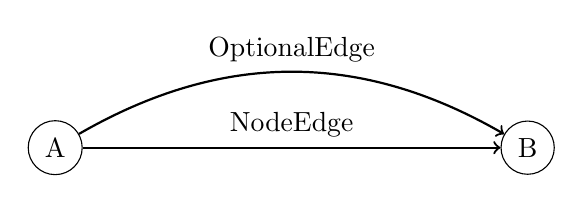
\begin{tikzpicture}
		\tikzset{vertex/.style = {shape=circle,draw,minimum size=.2em}}
		\tikzset{edge/.style = {->,> = latex'}}
		\node[vertex] (a) at  (0,0) {A};
		\node[vertex] (b) at  (6,0) {B};
		\path[->,draw,thick] (a) edge node[above] {NodeEdge} (b);
		\path[->,draw,thick, bend left] (a) edge node[above] {OptionalEdge} (b);
	\end{tikzpicture}
    \caption{Diagramm eines optionalen Sequenz-Knotens}
    \label{FIG:DiagramOptionalNode}
  \end{subfigure}
  \begin{subfigure}[c]{0.49\textwidth}
    \lstinputlisting[language=Java,caption={Java-Interface aus einem optionalen Sequenz-Knoten},label={LST:JInterfaceOptionalNode}]{Scope_optional.java}
  \end{subfigure}
  \caption{Diagramm und Interface eines optionalen Sequenz-Knotens}
  \label{FIG:OptionalNode}
\end{figure}

\subsection{Kante mit Alternativen}
Alternativen in der EBNF können auf parallele Kanten vom selben Typ zwischen zwei Knoten abgebildet werden (siehe Abbildung~\ref{FIG:DiagramAlternativeNode}). Dadurch können beide Kanten analog wie bei einer Sequenz abgebildet werden, nur dass es einem Interface mehrere Methoden auftreten können (Listing~\ref{LST:JInterfaceAlternativeNode}). Die Interface-Typen und Rückgabewerte sind analog wie bei der Sequenz.
\begin{figure}[ht]
\centering
  \begin{subfigure}[c]{0.49\textwidth}
  	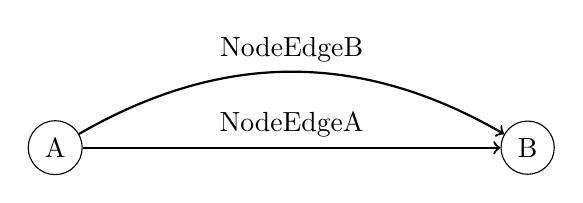
\begin{tikzpicture}
		\tikzset{vertex/.style = {shape=circle,draw,minimum size=.2em}}
		\tikzset{edge/.style = {->,> = latex'}}
		\node[vertex] (a) at  (0,0) {A};
		\node[vertex] (b) at  (6,0) {B};
		\path[->,draw,thick] (a) edge node[above] {NodeEdgeA} (b);
		\path[->,draw,thick, bend left] (a) edge node[above] {NodeEdgeB} (b);
	\end{tikzpicture}
    \caption{Diagramm alternativer Knoten}
    \label{FIG:DiagramAlternativeNode}
  \end{subfigure}
  \begin{subfigure}[c]{0.49\textwidth}
    \lstinputlisting[language=Java,caption={Java-Interface aus alternativen Knoten},label={LST:JInterfaceAlternativeNode}]{Scope_alternative.java}
  \end{subfigure}
  \caption{Diagramm und Interface alternativer Knotens}
  \label{FIG:AlternativeNode}
\end{figure}

\subsection{Kante mit optionaler Schleife}
Da die Wiederholung bei EBNF optional ist (beliebig oft oder keinmal auftreten darf), gibt es hier, wie beim optionalen Element eine parallele Kante vom Typ OptionalEdge.
Zusätzlich gibt es eine dritte Kante, die ebenfalls parallel ist aber in die entgegengesetzte Richtung zeigt. Diese Kante zeigt ebenfalls eine Vererbungsbeziehung an, um den Methodenaufruf von Interface A auch in Interface B verfügbar zu machen (Abbildung~\ref{FIG:DiagramLoopNode}).
\begin{figure}[ht]
\centering
  \begin{subfigure}[c]{0.49\textwidth}
  	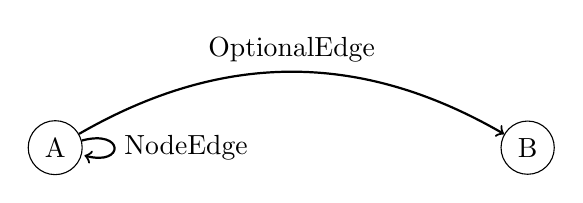
\begin{tikzpicture}
		\tikzset{vertex/.style = {shape=circle,draw,minimum size=.2em}}
		\tikzset{edge/.style = {->,> = latex'}}
		\node[vertex] (a) at  (0,0) {A};
		\node[vertex] (b) at  (6,0) {B};
		\path[->,draw,thick, bend left] (a) edge node[above] {OptionalEdge} (b);
		\path[->,draw,thick, loop right] (a) edge node[right] {NodeEdge} (a);
	\end{tikzpicture}
    \caption{Diagramm eines Schleifen-Knotens}
    \label{FIG:DiagramLoopNode}
  \end{subfigure}
  \begin{subfigure}[c]{0.49\textwidth}
    \lstinputlisting[language=Java,caption={Java-Interface aus einem Schleifen-Knoten},label={LST:JInterfaceLoopNode}]{Scope_loop.java}
  \end{subfigure}
  \caption{Diagramm und Interface eines Schleifen-Knotens}
  \label{FIG:LoopNode}
\end{figure}

\subsection{Sequenz von Knoten}
Tritt eine Sequenz von Knoten auf, muss für jeden Knoten ein Interface mit einer Methode generiert werden, um die Aufruf-Reihenfolge zu gewährleisten. Abbildung~\ref{FIG:SequenceNode} zeigt ein Beispiel mit zwei Knoten in einer Sequenz.
\begin{figure}[ht]
\centering
  \begin{subfigure}[c]{0.49\textwidth}
  	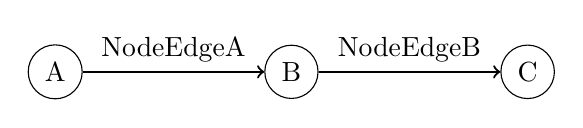
\begin{tikzpicture}
		\tikzset{vertex/.style = {shape=circle,draw,minimum size=.2em}}
		\tikzset{edge/.style = {->,> = latex'}}
		\node[vertex] (a) at  (0,0) {A};
		\node[vertex] (b) at  (3,0) {B};
		\node[vertex] (c) at  (6,0) {C};
		\path[->,draw,thick] (a) edge node[above] {NodeEdgeA} (b);
		\path[->,draw,thick] (b) edge node[above] {NodeEdgeB} (c);
	\end{tikzpicture}
    \caption{Diagramm einer Sequenz von Knoten}
    \label{FIG:DiagramSequenceNode}
  \end{subfigure}
  \begin{subfigure}[c]{0.49\textwidth}
    \lstinputlisting[language=Java,caption={Java-Interfaces aus einer Sequenz von Knoten},label={FIG:JInterfaceSequenceNode}]{Scope_sequence.java}
  \end{subfigure}
  \caption{Diagramm und Interface einer Sequenz von Knotens}
  \label{FIG:SequenceNode}
\end{figure}


\section{Schwierigkeiten beim Bau}
Beim Erstellen des Prototypen traten einige Schwierigkeiten auf. Die größten werden in diesem Abschnitt besprochen: die Behandlung der Rekursion der EBNF-Grammatik und die der Typen.

\subsection{Behandlung der Rekursion}

\subsection{Typen}

\subsubsection{Mapping auf Typen der Hostsprache}
- NTs -> Methoden (Einschränungen)

- Interfacenamen beliebig

\subsubsection{Generierung von Typen aus EBNF-Regeln}


\section{Einschränkungen bei der Grammatik}
Die EBNF-Grammatik kann nicht beliebig formuliert sein.

\subsection{Startregel}
In der Grammatik muss eine Startregel definiert sein, die nur ein Nicht-Terminal beinhaltet. Daraus wird das erste Interface als Einstiegspunkt generiert.

\subsection{Lexer-Regeln}
Für jede Lexer-Regel sollte es eine entsprechende Parser-Regel geben, die nur die jeweilige Lexer-Regel beinhaltet. Dadurch kann der Listener des Parsers die Typen auch verarbeiten.

Falls eine Regel innerhalb einer anderen vorkommt, ohne ein Trennsymbol zu einer anderen, darf es ebenfalls keine Lexer-Regel sein, um vom Listener erkannt zu werden.


\chapter{Testlauf mit anschaulichem Beispiel}


\section{Optimierungspotenzial}


\section{Varianten}


\end{document}
